\scanpage{105}
% archive foliation: 104
$\Pi_2(X,\xi)$

a) Si $X$ simplement connexe

alors
\[
M\unsure{\rightsquigarrow|\longmapsto}H^2(X,M)
\]
avec $M$ \deleted{\unsure{faisceau de}} \inserted{groupe de} torsion \deleted{\unsure{constant}} fini est exact à g., donc proreprésentable par
\[
H^2(X,M)=\operatorname{Hom\,cont}(\uline{\Pi_2(X)},M)
\]

b) Dans le cas général,
\diagram{\begin{tikzcd}[column sep=small,row sep=small]
\Pi_2(X,\xi)=\Pi_2(\widetilde{X(\xi)}) \arrow[d,phantom,shift right=3em] \arrow[d,shift right=4em] \\
\text{revêtement universel \unsure{pointé} défini par }\xi
\end{tikzcd}}

\figure{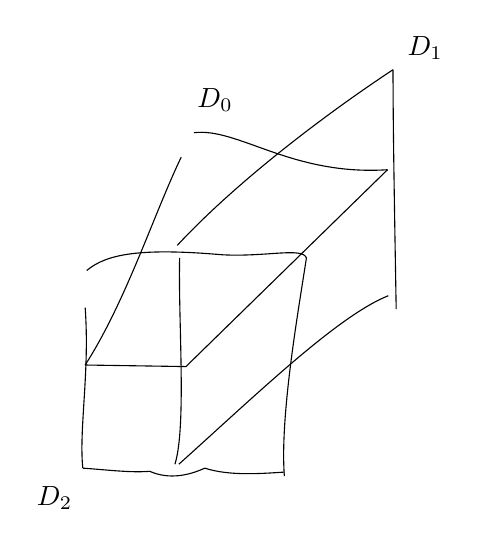
\begin{tikzpicture}[x=1cm,y=1cm]
\draw (0.05,0.12) .. controls (0.35,0.10) and (0.65,0.06) .. (0.90,0.08)
 .. controls (1.15,-0.03) and (1.40,0.03) .. (1.60,0.12);
\draw (1.60,0.12) .. controls (1.91,0.02) and (2.30,0.05) .. (2.61,0.07);
\draw (0.05,0.12) .. controls (0,0.62) and (0.14,1.35) .. (0.08,2.16);
\draw (2.61,0.02) .. controls (2.55,0.80) and (2.80,2.19) .. (2.89,2.79)
 .. controls (2.84,2.93) and (2.38,2.80) .. (1.82,2.83)
 .. controls (0.78,2.92) and (0.35,2.84) .. (0.10,2.63);
\draw (1.22,0.17) .. controls (1.37,0.65) and (1.26,2.03) .. (1.28,2.79);
\draw (1.25,2.95) .. controls (2.08,3.84) and (3.29,4.72) .. (3.99,5.18);
\draw (3.99,5.18) .. controls (3.99,4.40) and (4.01,3.34) .. (4.03,2.14);
\draw (1.27,0.17) .. controls (2.24,1.04) and (3.28,2.05) .. (3.93,2.31);
\draw (0.08,1.43) -- (1.36,1.41) -- (3.92,3.91);
\draw (0.08,1.43) .. controls (0.60,2.24) and (0.95,3.34) .. (1.30,4.07);
\draw (1.46,4.38) .. controls (2.02,4.45) and (2.70,3.83) .. (3.92,3.91);
\node[above] at (1.73,4.52) {$D_0$};
\node[above right] at (4.05,5.18) {$D_1$};
\node[below left] at (0.04,0.01) {$D_2$};
\end{tikzpicture}}

\figure{\begin{tikzpicture}
\begin{scope}[rotate=180,transform shape]
\node at (0,0) {$\mathbf T(\mathbf E_1,\ldots,\mathbf E_n)^{\deleted{\unsure{\Phi}}}$};
\node at (3.25,0.05) {$\deleted{\unsure{E}}\quad\mathcal F$};
\node at (-2.9,-0.67) {$\mathbf X$};
\node at (-1.70,-1.12) {$\mathbf K$};
\node at (-0.67,-0.63) {$\deleted{\unsure{\pi}}$};
\node at (-0.60,-0.92) {$p_1$};
\node at (0.55,-0.92) {$p_n$};
\node at (0.75,-2.03) {$\mathbf G_1\times\cdots\times\mathbf G_n$};
\node at (3.27,-1.99) {$\unsure{\mathcal K}$};
\end{scope}
\end{tikzpicture}}
